\documentclass[1p]{elsarticle_modified}
%\bibliographystyle{elsarticle-num}

%\usepackage[colorlinks]{hyperref}
%\usepackage{abbrmath_seonhwa} %\Abb, \Ascr, \Acal ,\Abf, \Afrak
\usepackage{amsfonts}
\usepackage{amssymb}
\usepackage{amsmath}
\usepackage{amsthm}
\usepackage{scalefnt}
\usepackage{amsbsy}
\usepackage{kotex}
\usepackage{caption}
\usepackage{subfig}
\usepackage{color}
\usepackage{graphicx}
\usepackage{xcolor} %% white, black, red, green, blue, cyan, magenta, yellow
\usepackage{float}
\usepackage{setspace}
\usepackage{hyperref}

\usepackage{tikz}
\usetikzlibrary{arrows}

\usepackage{multirow}
\usepackage{array} % fixed length table
\usepackage{hhline}

%%%%%%%%%%%%%%%%%%%%%
\makeatletter
\renewcommand*\env@matrix[1][\arraystretch]{%
	\edef\arraystretch{#1}%
	\hskip -\arraycolsep
	\let\@ifnextchar\new@ifnextchar
	\array{*\c@MaxMatrixCols c}}
\makeatother %https://tex.stackexchange.com/questions/14071/how-can-i-increase-the-line-spacing-in-a-matrix
%%%%%%%%%%%%%%%

\usepackage[normalem]{ulem}

\newcommand{\msout}[1]{\ifmmode\text{\sout{\ensuremath{#1}}}\else\sout{#1}\fi}
%SOURCE: \msout is \stkout macro in https://tex.stackexchange.com/questions/20609/strikeout-in-math-mode

\newcommand{\cancel}[1]{
	\ifmmode
	{\color{red}\msout{#1}}
	\else
	{\color{red}\sout{#1}}
	\fi
}

\newcommand{\add}[1]{
	{\color{blue}\uwave{#1}}
}

\newcommand{\replace}[2]{
	\ifmmode
	{\color{red}\msout{#1}}{\color{blue}\uwave{#2}}
	\else
	{\color{red}\sout{#1}}{\color{blue}\uwave{#2}}
	\fi
}

\newcommand{\Sol}{\mathcal{S}} %segment
\newcommand{\D}{D} %diagram
\newcommand{\A}{\mathcal{A}} %arc


%%%%%%%%%%%%%%%%%%%%%%%%%%%%%5 test

\def\sl{\operatorname{\textup{SL}}(2,\Cbb)}
\def\psl{\operatorname{\textup{PSL}}(2,\Cbb)}
\def\quan{\mkern 1mu \triangleright \mkern 1mu}

\theoremstyle{definition}
\newtheorem{thm}{Theorem}[section]
\newtheorem{prop}[thm]{Proposition}
\newtheorem{lem}[thm]{Lemma}
\newtheorem{ques}[thm]{Question}
\newtheorem{cor}[thm]{Corollary}
\newtheorem{defn}[thm]{Definition}
\newtheorem{exam}[thm]{Example}
\newtheorem{rmk}[thm]{Remark}
\newtheorem{alg}[thm]{Algorithm}

\newcommand{\I}{\sqrt{-1}}
\begin{document}

%\begin{frontmatter}
%
%\title{Boundary parabolic representations of knots up to 8 crossings}
%
%%% Group authors per affiliation:
%\author{Yunhi Cho} 
%\address{Department of Mathematics, University of Seoul, Seoul, Korea}
%\ead{yhcho@uos.ac.kr}
%
%
%\author{Seonhwa Kim} %\fnref{s_kim}}
%\address{Center for Geometry and Physics, Institute for Basic Science, Pohang, 37673, Korea}
%\ead{ryeona17@ibs.re.kr}
%
%\author{Hyuk Kim}
%\address{Department of Mathematical Sciences, Seoul National University, Seoul 08826, Korea}
%\ead{hyukkim@snu.ac.kr}
%
%\author{Seokbeom Yoon}
%\address{Department of Mathematical Sciences, Seoul National University, Seoul, 08826,  Korea}
%\ead{sbyoon15@snu.ac.kr}
%
%\begin{abstract}
%We find all boundary parabolic representation of knots up to 8 crossings.
%
%\end{abstract}
%\begin{keyword}
%    \MSC[2010] 57M25 
%\end{keyword}
%
%\end{frontmatter}

%\linenumbers
%\tableofcontents
%
\newcommand\colored[1]{\textcolor{white}{\rule[-0.35ex]{0.8em}{1.4ex}}\kern-0.8em\color{red} #1}%
%\newcommand\colored[1]{\textcolor{white}{ #1}\kern-2.17ex	\textcolor{white}{ #1}\kern-1.81ex	\textcolor{white}{ #1}\kern-2.15ex\color{red}#1	}

{\Large $\underline{12n_{0850}~(K12n_{0850})}$}

\setlength{\tabcolsep}{10pt}
\renewcommand{\arraystretch}{1.6}
\vspace{1cm}\begin{tabular}{m{100pt}>{\centering\arraybackslash}m{274pt}}
\multirow{5}{120pt}{
	\centering
	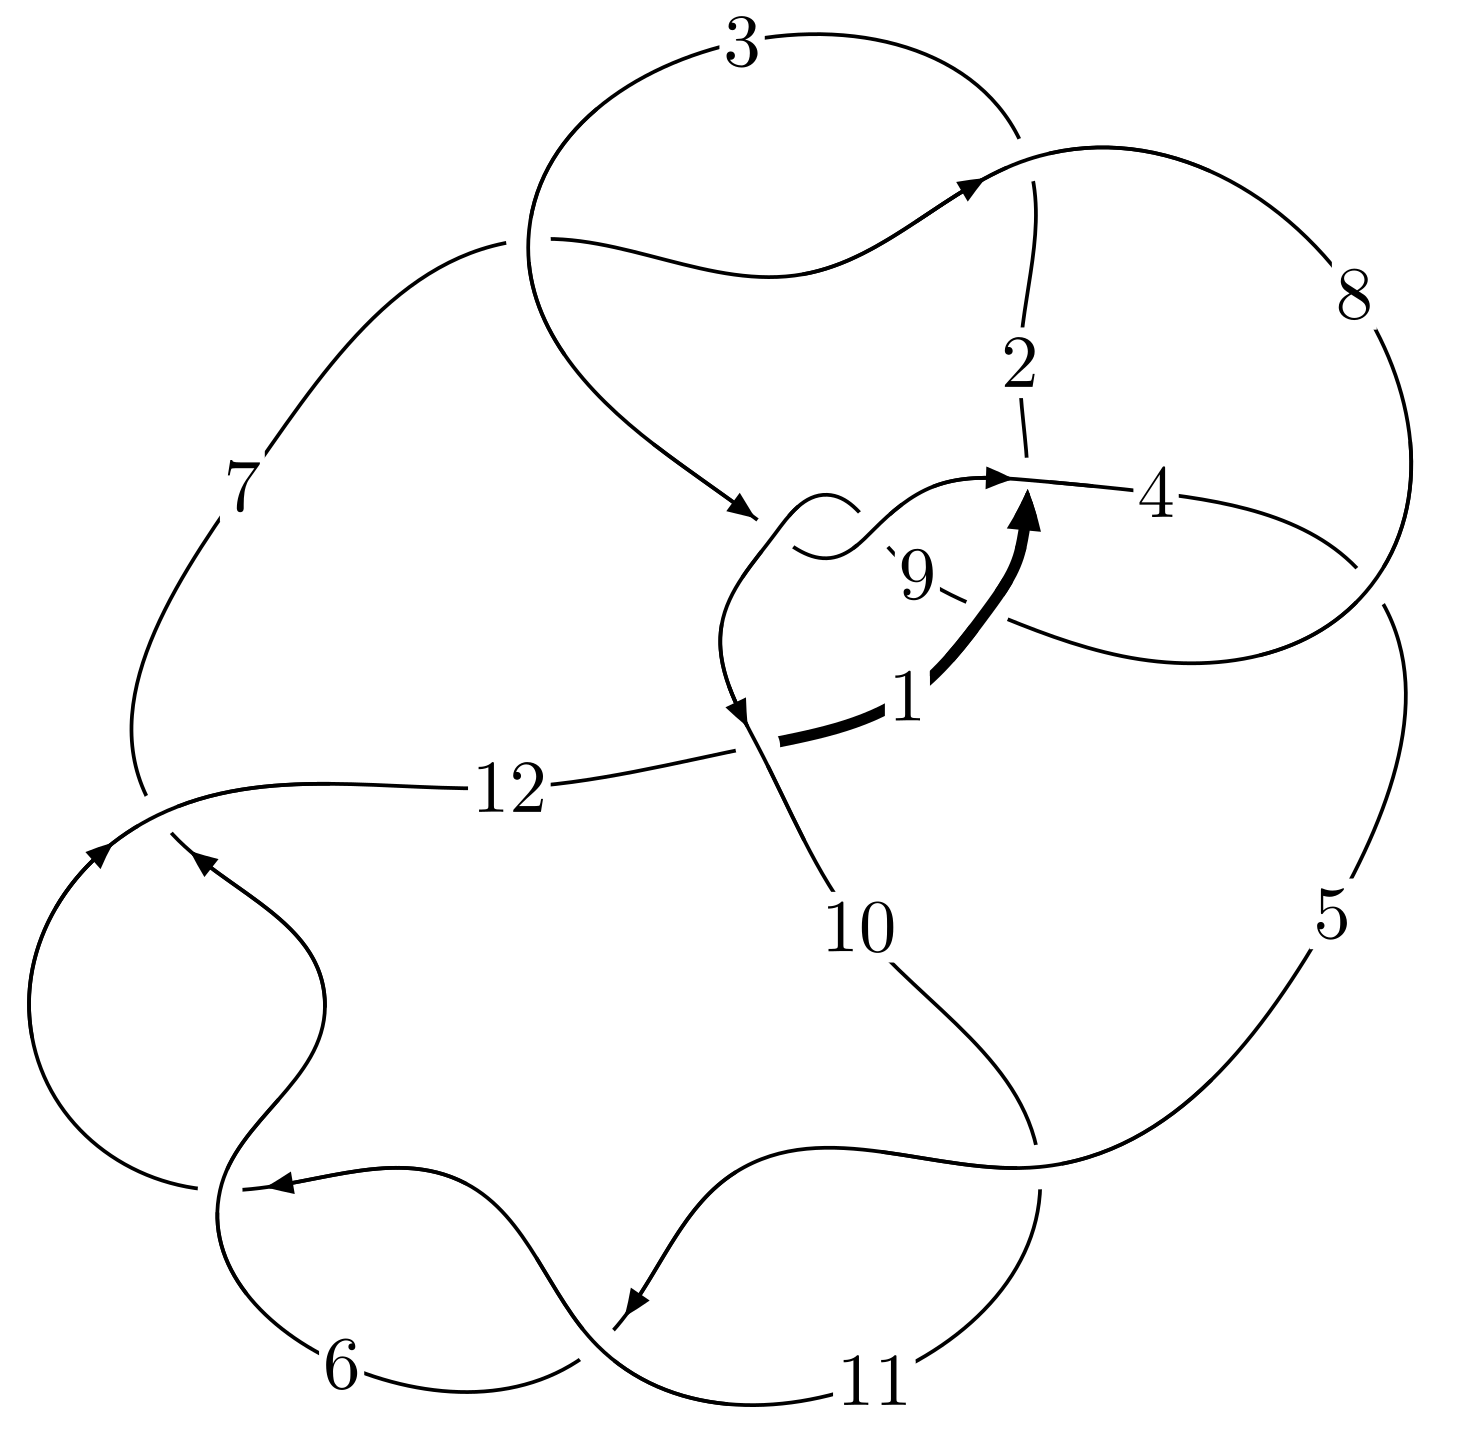
\includegraphics[width=112pt]{../../../GIT/diagram.site/Diagrams/png/2939_12n_0850.png}\\
\ \ \ A knot diagram\footnotemark}&
\allowdisplaybreaks
\textbf{Linearized knot diagam} \\
\cline{2-2}
 &
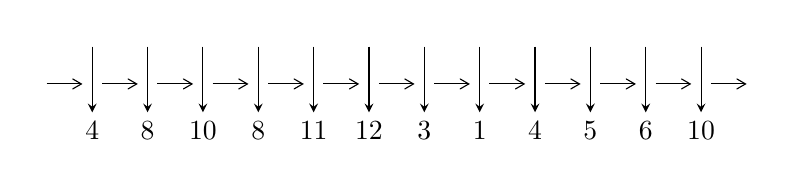
\begin{tikzpicture}[x=20pt, y=17pt]
	% nodes
	\node (C0) at (0, 0) {};
	\node (C1) at (1, 0) {};
	\node (C1U) at (1, +1) {};
	\node (C1D) at (1, -1) {4};

	\node (C2) at (2, 0) {};
	\node (C2U) at (2, +1) {};
	\node (C2D) at (2, -1) {8};

	\node (C3) at (3, 0) {};
	\node (C3U) at (3, +1) {};
	\node (C3D) at (3, -1) {10};

	\node (C4) at (4, 0) {};
	\node (C4U) at (4, +1) {};
	\node (C4D) at (4, -1) {8};

	\node (C5) at (5, 0) {};
	\node (C5U) at (5, +1) {};
	\node (C5D) at (5, -1) {11};

	\node (C6) at (6, 0) {};
	\node (C6U) at (6, +1) {};
	\node (C6D) at (6, -1) {12};

	\node (C7) at (7, 0) {};
	\node (C7U) at (7, +1) {};
	\node (C7D) at (7, -1) {3};

	\node (C8) at (8, 0) {};
	\node (C8U) at (8, +1) {};
	\node (C8D) at (8, -1) {1};

	\node (C9) at (9, 0) {};
	\node (C9U) at (9, +1) {};
	\node (C9D) at (9, -1) {4};

	\node (C10) at (10, 0) {};
	\node (C10U) at (10, +1) {};
	\node (C10D) at (10, -1) {5};

	\node (C11) at (11, 0) {};
	\node (C11U) at (11, +1) {};
	\node (C11D) at (11, -1) {6};

	\node (C12) at (12, 0) {};
	\node (C12U) at (12, +1) {};
	\node (C12D) at (12, -1) {10};
	\node (C13) at (13, 0) {};

	% arrows
	\draw[->,>={angle 60}]
	(C0) edge (C1) (C1) edge (C2) (C2) edge (C3) (C3) edge (C4) (C4) edge (C5) (C5) edge (C6) (C6) edge (C7) (C7) edge (C8) (C8) edge (C9) (C9) edge (C10) (C10) edge (C11) (C11) edge (C12) (C12) edge (C13) ;	\draw[->,>=stealth]
	(C1U) edge (C1D) (C2U) edge (C2D) (C3U) edge (C3D) (C4U) edge (C4D) (C5U) edge (C5D) (C6U) edge (C6D) (C7U) edge (C7D) (C8U) edge (C8D) (C9U) edge (C9D) (C10U) edge (C10D) (C11U) edge (C11D) (C12U) edge (C12D) ;
	\end{tikzpicture} \\
\hhline{~~} \\& 
\textbf{Solving Sequence} \\ \cline{2-2} 
 &
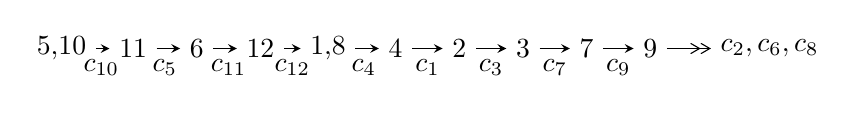
\begin{tikzpicture}[x=23pt, y=7pt]
	% node
	\node (A0) at (-1/8, 0) {5,10};
	\node (A1) at (1, 0) {11};
	\node (A2) at (2, 0) {6};
	\node (A3) at (3, 0) {12};
	\node (A4) at (65/16, 0) {1,8};
	\node (A5) at (41/8, 0) {4};
	\node (A6) at (49/8, 0) {2};
	\node (A7) at (57/8, 0) {3};
	\node (A8) at (65/8, 0) {7};
	\node (A9) at (73/8, 0) {9};
	\node (C1) at (1/2, -1) {$c_{10}$};
	\node (C2) at (3/2, -1) {$c_{5}$};
	\node (C3) at (5/2, -1) {$c_{11}$};
	\node (C4) at (7/2, -1) {$c_{12}$};
	\node (C5) at (37/8, -1) {$c_{4}$};
	\node (C6) at (45/8, -1) {$c_{1}$};
	\node (C7) at (53/8, -1) {$c_{3}$};
	\node (C8) at (61/8, -1) {$c_{7}$};
	\node (C9) at (69/8, -1) {$c_{9}$};
	\node (A10) at (11, 0) {$c_{2},c_{6},c_{8}$};

	% edge
	\draw[->,>=stealth]	
	(A0) edge (A1) (A1) edge (A2) (A2) edge (A3) (A3) edge (A4) (A4) edge (A5) (A5) edge (A6) (A6) edge (A7) (A7) edge (A8) (A8) edge (A9) ;
	\draw[->>,>={angle 60}]	
	(A9) edge (A10);
\end{tikzpicture} \\ 

\end{tabular} \\

\footnotetext{
The image of knot diagram is generated by the software ``\textbf{Draw programme}" developed by Andrew Bartholomew(\url{http://www.layer8.co.uk/maths/draw/index.htm\#Running-draw}), where we modified some parts for our purpose(\url{https://github.com/CATsTAILs/LinksPainter}).
}\phantom \\ \newline 
\centering \textbf{Ideals for irreducible components\footnotemark of $X_{\text{par}}$} 
 
\begin{align*}
I^u_{1}&=\langle 
- u^{10}-5 u^9-4 u^8+8 u^7- u^6-16 u^5+19 u^4+20 u^3-15 u^2+2 b+5 u+4,\\
\phantom{I^u_{1}}&\phantom{= \langle  }-3 u^{10}-10 u^9- u^8+14 u^7-17 u^6-17 u^5+47 u^4+13 u^3-25 u^2+2 a+18 u+7,\\
\phantom{I^u_{1}}&\phantom{= \langle  }u^{11}+5 u^{10}+6 u^9-4 u^8-3 u^7+14 u^6-5 u^5-30 u^4- u^3+9 u^2-10 u-4\rangle \\
I^u_{2}&=\langle 
- u^5+4 u^3+b-3 u,\;u^5-5 u^3+u^2+a+6 u-3,\;u^7- u^6-5 u^5+5 u^4+6 u^3-7 u^2+u+1\rangle \\
I^u_{3}&=\langle 
b,\;a+1,\;u+1\rangle \\
I^u_{4}&=\langle 
- a^3+b+a+1,\;a^4+a^3-2 a-1,\;u-1\rangle \\
\\
\end{align*}
\raggedright * 4 irreducible components of $\dim_{\mathbb{C}}=0$, with total 23 representations.\\
\footnotetext{All coefficients of polynomials are rational numbers. But the coefficients are sometimes approximated in decimal forms when there is not enough margin.}
\newpage
\renewcommand{\arraystretch}{1}
\centering \section*{I. $I^u_{1}= \langle - u^{10}-5 u^9+\cdots+2 b+4,\;-3 u^{10}-10 u^9+\cdots+2 a+7,\;u^{11}+5 u^{10}+\cdots-10 u-4 \rangle$}
\flushleft \textbf{(i) Arc colorings}\\
\begin{tabular}{m{7pt} m{180pt} m{7pt} m{180pt} }
\flushright $a_{5}=$&$\begin{pmatrix}0\\u\end{pmatrix}$ \\
\flushright $a_{10}=$&$\begin{pmatrix}1\\0\end{pmatrix}$ \\
\flushright $a_{11}=$&$\begin{pmatrix}1\\u^2\end{pmatrix}$ \\
\flushright $a_{6}=$&$\begin{pmatrix}- u\\- u^3+u\end{pmatrix}$ \\
\flushright $a_{12}=$&$\begin{pmatrix}- u^2+1\\- u^4+2 u^2\end{pmatrix}$ \\
\flushright $a_{1}=$&$\begin{pmatrix}u^4-3 u^2+1\\- u^4+2 u^2\end{pmatrix}$ \\
\flushright $a_{8}=$&$\begin{pmatrix}\frac{3}{2} u^{10}+5 u^9+\cdots-9 u-\frac{7}{2}\\\frac{1}{2} u^{10}+\frac{5}{2} u^9+\cdots-\frac{5}{2} u-2\end{pmatrix}$ \\
\flushright $a_{4}=$&$\begin{pmatrix}\frac{1}{4} u^{10}+\frac{3}{4} u^9+\cdots-\frac{5}{4} u-1\\-\frac{1}{2} u^{10}-\frac{3}{2} u^9+\cdots+\frac{5}{2} u+1\end{pmatrix}$ \\
\flushright $a_{2}=$&$\begin{pmatrix}-\frac{1}{2} u^9-\frac{1}{2} u^8+\cdots+\frac{1}{2} u+\frac{3}{2}\\\frac{5}{2} u^{10}+\frac{17}{2} u^9+\cdots-\frac{23}{2} u-6\end{pmatrix}$ \\
\flushright $a_{3}=$&$\begin{pmatrix}-\frac{1}{4} u^{10}-\frac{3}{4} u^9+\cdots-\frac{3}{4} u^2+\frac{5}{4} u\\-\frac{1}{2} u^{10}-\frac{3}{2} u^9+\cdots+\frac{5}{2} u+1\end{pmatrix}$ \\
\flushright $a_{7}=$&$\begin{pmatrix}u^3-2 u\\u^5-3 u^3+u\end{pmatrix}$ \\
\flushright $a_{9}=$&$\begin{pmatrix}- u^{10}-\frac{5}{2} u^9+\cdots+\frac{7}{2} u+\frac{5}{2}\\-\frac{1}{2} u^{10}-\frac{5}{2} u^9+\cdots+\frac{7}{2} u+2\end{pmatrix}$\\&\end{tabular}
\flushleft \textbf{(ii) Obstruction class $= -1$}\\~\\
\flushleft \textbf{(iii) Cusp Shapes $= -7 u^{10}-25 u^9-6 u^8+36 u^7-35 u^6-50 u^5+113 u^4+43 u^3-65 u^2+46 u+2$}\\~\\
\newpage\renewcommand{\arraystretch}{1}
\flushleft \textbf{(iv) u-Polynomials at the component}\newline \\
\begin{tabular}{m{50pt}|m{274pt}}
Crossings & \hspace{64pt}u-Polynomials at each crossing \\
\hline $$\begin{aligned}c_{1}\end{aligned}$$&$\begin{aligned}
&u^{11}-7 u^{10}+\cdots-2 u+2
\end{aligned}$\\
\hline $$\begin{aligned}c_{2},c_{3},c_{7}\\c_{9}\end{aligned}$$&$\begin{aligned}
&u^{11}+14 u^9+4 u^8+46 u^7+67 u^6-66 u^5-7 u^4-30 u^3-9 u^2-3 u-1
\end{aligned}$\\
\hline $$\begin{aligned}c_{4},c_{8}\end{aligned}$$&$\begin{aligned}
&u^{11}+u^{10}+\cdots-4 u-1
\end{aligned}$\\
\hline $$\begin{aligned}c_{5},c_{6},c_{10}\\c_{11}\end{aligned}$$&$\begin{aligned}
&u^{11}+5 u^{10}+\cdots-10 u-4
\end{aligned}$\\
\hline $$\begin{aligned}c_{12}\end{aligned}$$&$\begin{aligned}
&u^{11}-3 u^{10}+\cdots-3192 u-576
\end{aligned}$\\
\hline
\end{tabular}\\~\\
\newpage\renewcommand{\arraystretch}{1}
\flushleft \textbf{(v) Riley Polynomials at the component}\newline \\
\begin{tabular}{m{50pt}|m{274pt}}
Crossings & \hspace{64pt}Riley Polynomials at each crossing \\
\hline $$\begin{aligned}c_{1}\end{aligned}$$&$\begin{aligned}
&y^{11}-31 y^{10}+\cdots+200 y-4
\end{aligned}$\\
\hline $$\begin{aligned}c_{2},c_{3},c_{7}\\c_{9}\end{aligned}$$&$\begin{aligned}
&y^{11}+28 y^{10}+\cdots-9 y-1
\end{aligned}$\\
\hline $$\begin{aligned}c_{4},c_{8}\end{aligned}$$&$\begin{aligned}
&y^{11}+17 y^{10}+\cdots+24 y-1
\end{aligned}$\\
\hline $$\begin{aligned}c_{5},c_{6},c_{10}\\c_{11}\end{aligned}$$&$\begin{aligned}
&y^{11}-13 y^{10}+\cdots+172 y-16
\end{aligned}$\\
\hline $$\begin{aligned}c_{12}\end{aligned}$$&$\begin{aligned}
&y^{11}+67 y^{10}+\cdots+7508160 y-331776
\end{aligned}$\\
\hline
\end{tabular}\\~\\
\newpage\flushleft \textbf{(vi) Complex Volumes and Cusp Shapes}
$$\begin{array}{c|c|c}  
\text{Solutions to }I^u_{1}& \I (\text{vol} + \sqrt{-1}CS) & \text{Cusp shape}\\
 \hline 
\begin{aligned}
u &= \phantom{-}1.18814\phantom{ +0.000000I} \\
a &= \phantom{-}0.348347\phantom{ +0.000000I} \\
b &= -0.566087\phantom{ +0.000000I}\end{aligned}
 & -5.45154\phantom{ +0.000000I} & -15.3520\phantom{ +0.000000I} \\ \hline\begin{aligned}
u &= \phantom{-}0.651462 + 1.063750 I \\
a &= \phantom{-}1.81578 + 0.65642 I \\
b &= -1.77237 + 0.06609 I\end{aligned}
 & \phantom{-}12.65630 - 3.45618 I & -10.65599 + 2.10885 I \\ \hline\begin{aligned}
u &= \phantom{-}0.651462 - 1.063750 I \\
a &= \phantom{-}1.81578 - 0.65642 I \\
b &= -1.77237 - 0.06609 I\end{aligned}
 & \phantom{-}12.65630 + 3.45618 I & -10.65599 - 2.10885 I \\ \hline\begin{aligned}
u &= \phantom{-}0.496165 + 0.539201 I \\
a &= -1.042860 - 0.661841 I \\
b &= \phantom{-}1.138470 - 0.357731 I\end{aligned}
 & \phantom{-}2.08534 - 1.86536 I & -10.69284 + 5.33447 I \\ \hline\begin{aligned}
u &= \phantom{-}0.496165 - 0.539201 I \\
a &= -1.042860 + 0.661841 I \\
b &= \phantom{-}1.138470 + 0.357731 I\end{aligned}
 & \phantom{-}2.08534 + 1.86536 I & -10.69284 - 5.33447 I \\ \hline\begin{aligned}
u &= -1.53157 + 0.15203 I \\
a &= -0.354779 + 0.587363 I \\
b &= \phantom{-}1.12977 + 1.06011 I\end{aligned}
 & -4.66784 + 4.30939 I & -14.0390 - 6.9085 I \\ \hline\begin{aligned}
u &= -1.53157 - 0.15203 I \\
a &= -0.354779 - 0.587363 I \\
b &= \phantom{-}1.12977 - 1.06011 I\end{aligned}
 & -4.66784 - 4.30939 I & -14.0390 + 6.9085 I \\ \hline\begin{aligned}
u &= -0.330126\phantom{ +0.000000I} \\
a &= \phantom{-}0.768686\phantom{ +0.000000I} \\
b &= -0.139205\phantom{ +0.000000I}\end{aligned}
 & -0.487897\phantom{ +0.000000I} & -20.3390\phantom{ +0.000000I} \\ \hline\begin{aligned}
u &= -1.64929 + 0.39522 I \\
a &= \phantom{-}0.914271 - 0.873133 I \\
b &= -1.77328 - 0.21395 I\end{aligned}
 & \phantom{-}5.23140 + 8.93346 I & -13.21655 - 3.59394 I \\ \hline\begin{aligned}
u &= -1.64929 - 0.39522 I \\
a &= \phantom{-}0.914271 + 0.873133 I \\
b &= -1.77328 + 0.21395 I\end{aligned}
 & \phantom{-}5.23140 - 8.93346 I & -13.21655 + 3.59394 I\\
 \hline 
 \end{array}$$\newpage$$\begin{array}{c|c|c}  
\text{Solutions to }I^u_{1}& \I (\text{vol} + \sqrt{-1}CS) & \text{Cusp shape}\\
 \hline 
\begin{aligned}
u &= -1.79155\phantom{ +0.000000I} \\
a &= \phantom{-}0.218139\phantom{ +0.000000I} \\
b &= -0.739878\phantom{ +0.000000I}\end{aligned}
 & -16.4464\phantom{ +0.000000I} & -7.09980\phantom{ +0.000000I}\\
 \hline 
 \end{array}$$\newpage\newpage\renewcommand{\arraystretch}{1}
\centering \section*{II. $I^u_{2}= \langle - u^5+4 u^3+b-3 u,\;u^5-5 u^3+u^2+a+6 u-3,\;u^7- u^6-5 u^5+5 u^4+6 u^3-7 u^2+u+1 \rangle$}
\flushleft \textbf{(i) Arc colorings}\\
\begin{tabular}{m{7pt} m{180pt} m{7pt} m{180pt} }
\flushright $a_{5}=$&$\begin{pmatrix}0\\u\end{pmatrix}$ \\
\flushright $a_{10}=$&$\begin{pmatrix}1\\0\end{pmatrix}$ \\
\flushright $a_{11}=$&$\begin{pmatrix}1\\u^2\end{pmatrix}$ \\
\flushright $a_{6}=$&$\begin{pmatrix}- u\\- u^3+u\end{pmatrix}$ \\
\flushright $a_{12}=$&$\begin{pmatrix}- u^2+1\\- u^4+2 u^2\end{pmatrix}$ \\
\flushright $a_{1}=$&$\begin{pmatrix}u^4-3 u^2+1\\- u^4+2 u^2\end{pmatrix}$ \\
\flushright $a_{8}=$&$\begin{pmatrix}- u^5+5 u^3- u^2-6 u+3\\u^5-4 u^3+3 u\end{pmatrix}$ \\
\flushright $a_{4}=$&$\begin{pmatrix}- u^6+u^5+4 u^4-5 u^3-2 u^2+7 u-4\\u^4-3 u^2+1\end{pmatrix}$ \\
\flushright $a_{2}=$&$\begin{pmatrix}-2 u^6+2 u^5+10 u^4-10 u^3-11 u^2+14 u-4\\u^6-5 u^4+u^3+6 u^2-3 u\end{pmatrix}$ \\
\flushright $a_{3}=$&$\begin{pmatrix}- u^6+u^5+5 u^4-5 u^3-5 u^2+7 u-3\\u^4-3 u^2+1\end{pmatrix}$ \\
\flushright $a_{7}=$&$\begin{pmatrix}u^3-2 u\\u^5-3 u^3+u\end{pmatrix}$ \\
\flushright $a_{9}=$&$\begin{pmatrix}- u^5+5 u^3- u^2-6 u+4\\- u^3+2 u\end{pmatrix}$\\&\end{tabular}
\flushleft \textbf{(ii) Obstruction class $= 1$}\\~\\
\flushleft \textbf{(iii) Cusp Shapes $= 2 u^6-2 u^5-12 u^4+5 u^3+16 u^2-3 u-10$}\\~\\
\newpage\renewcommand{\arraystretch}{1}
\flushleft \textbf{(iv) u-Polynomials at the component}\newline \\
\begin{tabular}{m{50pt}|m{274pt}}
Crossings & \hspace{64pt}u-Polynomials at each crossing \\
\hline $$\begin{aligned}c_{1}\end{aligned}$$&$\begin{aligned}
&u^7-6 u^6+12 u^5-11 u^4+7 u^3-3 u^2-1
\end{aligned}$\\
\hline $$\begin{aligned}c_{2},c_{9}\end{aligned}$$&$\begin{aligned}
&u^7- u^6+u^5-2 u^4- u^2+1
\end{aligned}$\\
\hline $$\begin{aligned}c_{3},c_{7}\end{aligned}$$&$\begin{aligned}
&u^7+u^6+u^5+2 u^4+u^2-1
\end{aligned}$\\
\hline $$\begin{aligned}c_{4},c_{8}\end{aligned}$$&$\begin{aligned}
&u^7- u^5-2 u^3+u^2- u+1
\end{aligned}$\\
\hline $$\begin{aligned}c_{5},c_{6}\end{aligned}$$&$\begin{aligned}
&u^7+u^6-5 u^5-5 u^4+6 u^3+7 u^2+u-1
\end{aligned}$\\
\hline $$\begin{aligned}c_{10},c_{11}\end{aligned}$$&$\begin{aligned}
&u^7- u^6-5 u^5+5 u^4+6 u^3-7 u^2+u+1
\end{aligned}$\\
\hline $$\begin{aligned}c_{12}\end{aligned}$$&$\begin{aligned}
&u^7-5 u^6+7 u^5-5 u^4-4 u^3-7 u^2+5 u+1
\end{aligned}$\\
\hline
\end{tabular}\\~\\
\newpage\renewcommand{\arraystretch}{1}
\flushleft \textbf{(v) Riley Polynomials at the component}\newline \\
\begin{tabular}{m{50pt}|m{274pt}}
Crossings & \hspace{64pt}Riley Polynomials at each crossing \\
\hline $$\begin{aligned}c_{1}\end{aligned}$$&$\begin{aligned}
&y^7-12 y^6+26 y^5+11 y^4-29 y^3-31 y^2-6 y-1
\end{aligned}$\\
\hline $$\begin{aligned}c_{2},c_{3},c_{7}\\c_{9}\end{aligned}$$&$\begin{aligned}
&y^7+y^6-3 y^5-6 y^4-2 y^3+3 y^2+2 y-1
\end{aligned}$\\
\hline $$\begin{aligned}c_{4},c_{8}\end{aligned}$$&$\begin{aligned}
&y^7-2 y^6-3 y^5+2 y^4+6 y^3+3 y^2- y-1
\end{aligned}$\\
\hline $$\begin{aligned}c_{5},c_{6},c_{10}\\c_{11}\end{aligned}$$&$\begin{aligned}
&y^7-11 y^6+47 y^5-97 y^4+98 y^3-47 y^2+15 y-1
\end{aligned}$\\
\hline $$\begin{aligned}c_{12}\end{aligned}$$&$\begin{aligned}
&y^7-11 y^6-9 y^5-141 y^4+26 y^3-79 y^2+39 y-1
\end{aligned}$\\
\hline
\end{tabular}\\~\\
\newpage\flushleft \textbf{(vi) Complex Volumes and Cusp Shapes}
$$\begin{array}{c|c|c}  
\text{Solutions to }I^u_{2}& \I (\text{vol} + \sqrt{-1}CS) & \text{Cusp shape}\\
 \hline 
\begin{aligned}
u &= \phantom{-}0.602602 + 0.366097 I \\
a &= -0.802378 - 0.958802 I \\
b &= \phantom{-}1.74200 - 0.23095 I\end{aligned}
 & \phantom{-}3.42389 - 1.23175 I & -6.47743 + 5.11160 I \\ \hline\begin{aligned}
u &= \phantom{-}0.602602 - 0.366097 I \\
a &= -0.802378 + 0.958802 I \\
b &= \phantom{-}1.74200 + 0.23095 I\end{aligned}
 & \phantom{-}3.42389 + 1.23175 I & -6.47743 - 5.11160 I \\ \hline\begin{aligned}
u &= \phantom{-}1.50894\phantom{ +0.000000I} \\
a &= \phantom{-}1.02523\phantom{ +0.000000I} \\
b &= -1.39324\phantom{ +0.000000I}\end{aligned}
 & -10.4234\phantom{ +0.000000I} & -15.1670\phantom{ +0.000000I} \\ \hline\begin{aligned}
u &= -1.59539 + 0.14916 I \\
a &= -0.285687 + 0.511963 I \\
b &= \phantom{-}1.59460 + 0.65214 I\end{aligned}
 & -4.17528 + 3.26775 I & -10.72162 - 1.02180 I \\ \hline\begin{aligned}
u &= -1.59539 - 0.14916 I \\
a &= -0.285687 - 0.511963 I \\
b &= \phantom{-}1.59460 - 0.65214 I\end{aligned}
 & -4.17528 - 3.26775 I & -10.72162 + 1.02180 I \\ \hline\begin{aligned}
u &= -0.293328\phantom{ +0.000000I} \\
a &= \phantom{-}4.54991\phantom{ +0.000000I} \\
b &= -0.781203\phantom{ +0.000000I}\end{aligned}
 & -4.14361\phantom{ +0.000000I} & -7.95280\phantom{ +0.000000I} \\ \hline\begin{aligned}
u &= \phantom{-}1.76997\phantom{ +0.000000I} \\
a &= -0.399006\phantom{ +0.000000I} \\
b &= \phantom{-}0.501243\phantom{ +0.000000I}\end{aligned}
 & -16.8289\phantom{ +0.000000I} & -28.4820\phantom{ +0.000000I}\\
 \hline 
 \end{array}$$\newpage\newpage\renewcommand{\arraystretch}{1}
\centering \section*{III. $I^u_{3}= \langle b,\;a+1,\;u+1 \rangle$}
\flushleft \textbf{(i) Arc colorings}\\
\begin{tabular}{m{7pt} m{180pt} m{7pt} m{180pt} }
\flushright $a_{5}=$&$\begin{pmatrix}0\\-1\end{pmatrix}$ \\
\flushright $a_{10}=$&$\begin{pmatrix}1\\0\end{pmatrix}$ \\
\flushright $a_{11}=$&$\begin{pmatrix}1\\1\end{pmatrix}$ \\
\flushright $a_{6}=$&$\begin{pmatrix}1\\0\end{pmatrix}$ \\
\flushright $a_{12}=$&$\begin{pmatrix}0\\1\end{pmatrix}$ \\
\flushright $a_{1}=$&$\begin{pmatrix}-1\\1\end{pmatrix}$ \\
\flushright $a_{8}=$&$\begin{pmatrix}-1\\0\end{pmatrix}$ \\
\flushright $a_{4}=$&$\begin{pmatrix}-1\\-1\end{pmatrix}$ \\
\flushright $a_{2}=$&$\begin{pmatrix}-3\\-1\end{pmatrix}$ \\
\flushright $a_{3}=$&$\begin{pmatrix}-2\\-1\end{pmatrix}$ \\
\flushright $a_{7}=$&$\begin{pmatrix}1\\1\end{pmatrix}$ \\
\flushright $a_{9}=$&$\begin{pmatrix}0\\-1\end{pmatrix}$\\&\end{tabular}
\flushleft \textbf{(ii) Obstruction class $= 1$}\\~\\
\flushleft \textbf{(iii) Cusp Shapes $= -24$}\\~\\
\newpage\renewcommand{\arraystretch}{1}
\flushleft \textbf{(iv) u-Polynomials at the component}\newline \\
\begin{tabular}{m{50pt}|m{274pt}}
Crossings & \hspace{64pt}u-Polynomials at each crossing \\
\hline $$\begin{aligned}c_{1}\end{aligned}$$&$\begin{aligned}
&u-2
\end{aligned}$\\
\hline $$\begin{aligned}c_{2},c_{4},c_{8}\\c_{9},c_{10},c_{11}\\c_{12}\end{aligned}$$&$\begin{aligned}
&u+1
\end{aligned}$\\
\hline $$\begin{aligned}c_{3},c_{5},c_{6}\\c_{7}\end{aligned}$$&$\begin{aligned}
&u-1
\end{aligned}$\\
\hline
\end{tabular}\\~\\
\newpage\renewcommand{\arraystretch}{1}
\flushleft \textbf{(v) Riley Polynomials at the component}\newline \\
\begin{tabular}{m{50pt}|m{274pt}}
Crossings & \hspace{64pt}Riley Polynomials at each crossing \\
\hline $$\begin{aligned}c_{1}\end{aligned}$$&$\begin{aligned}
&y-4
\end{aligned}$\\
\hline $$\begin{aligned}c_{2},c_{3},c_{4}\\c_{5},c_{6},c_{7}\\c_{8},c_{9},c_{10}\\c_{11},c_{12}\end{aligned}$$&$\begin{aligned}
&y-1
\end{aligned}$\\
\hline
\end{tabular}\\~\\
\newpage\flushleft \textbf{(vi) Complex Volumes and Cusp Shapes}
$$\begin{array}{c|c|c}  
\text{Solutions to }I^u_{3}& \I (\text{vol} + \sqrt{-1}CS) & \text{Cusp shape}\\
 \hline 
\begin{aligned}
u &= -1.00000\phantom{ +0.000000I} \\
a &= -1.00000\phantom{ +0.000000I} \\
b &= \phantom{-0.000000 } 0\end{aligned}
 & -6.57974\phantom{ +0.000000I} & -24.0000\phantom{ +0.000000I}\\
 \hline 
 \end{array}$$\newpage\newpage\renewcommand{\arraystretch}{1}
\centering \section*{IV. $I^u_{4}= \langle - a^3+b+a+1,\;a^4+a^3-2 a-1,\;u-1 \rangle$}
\flushleft \textbf{(i) Arc colorings}\\
\begin{tabular}{m{7pt} m{180pt} m{7pt} m{180pt} }
\flushright $a_{5}=$&$\begin{pmatrix}0\\1\end{pmatrix}$ \\
\flushright $a_{10}=$&$\begin{pmatrix}1\\0\end{pmatrix}$ \\
\flushright $a_{11}=$&$\begin{pmatrix}1\\1\end{pmatrix}$ \\
\flushright $a_{6}=$&$\begin{pmatrix}-1\\0\end{pmatrix}$ \\
\flushright $a_{12}=$&$\begin{pmatrix}0\\1\end{pmatrix}$ \\
\flushright $a_{1}=$&$\begin{pmatrix}-1\\1\end{pmatrix}$ \\
\flushright $a_{8}=$&$\begin{pmatrix}a\\a^3- a-1\end{pmatrix}$ \\
\flushright $a_{4}=$&$\begin{pmatrix}a^2\\- a^3- a^2+a+2\end{pmatrix}$ \\
\flushright $a_{2}=$&$\begin{pmatrix}- a-2\\a^3-1\end{pmatrix}$ \\
\flushright $a_{3}=$&$\begin{pmatrix}- a^3+a+2\\- a^3- a^2+a+2\end{pmatrix}$ \\
\flushright $a_{7}=$&$\begin{pmatrix}-1\\-1\end{pmatrix}$ \\
\flushright $a_{9}=$&$\begin{pmatrix}- a^3+a+1\\2 a^3- a-2\end{pmatrix}$\\&\end{tabular}
\flushleft \textbf{(ii) Obstruction class $= -1$}\\~\\
\flushleft \textbf{(iii) Cusp Shapes $= -14$}\\~\\
\newpage\renewcommand{\arraystretch}{1}
\flushleft \textbf{(iv) u-Polynomials at the component}\newline \\
\begin{tabular}{m{50pt}|m{274pt}}
Crossings & \hspace{64pt}u-Polynomials at each crossing \\
\hline $$\begin{aligned}c_{1}\end{aligned}$$&$\begin{aligned}
&(u^2+u-1)^2
\end{aligned}$\\
\hline $$\begin{aligned}c_{2},c_{3},c_{7}\\c_{9}\end{aligned}$$&$\begin{aligned}
&u^4- u^3+2 u^2-4 u+1
\end{aligned}$\\
\hline $$\begin{aligned}c_{4},c_{8}\end{aligned}$$&$\begin{aligned}
&u^4+u^3-2 u-1
\end{aligned}$\\
\hline $$\begin{aligned}c_{5},c_{6},c_{10}\\c_{11}\end{aligned}$$&$\begin{aligned}
&(u-1)^4
\end{aligned}$\\
\hline $$\begin{aligned}c_{12}\end{aligned}$$&$\begin{aligned}
&(u+1)^4
\end{aligned}$\\
\hline
\end{tabular}\\~\\
\newpage\renewcommand{\arraystretch}{1}
\flushleft \textbf{(v) Riley Polynomials at the component}\newline \\
\begin{tabular}{m{50pt}|m{274pt}}
Crossings & \hspace{64pt}Riley Polynomials at each crossing \\
\hline $$\begin{aligned}c_{1}\end{aligned}$$&$\begin{aligned}
&(y^2-3 y+1)^2
\end{aligned}$\\
\hline $$\begin{aligned}c_{2},c_{3},c_{7}\\c_{9}\end{aligned}$$&$\begin{aligned}
&y^4+3 y^3-2 y^2-12 y+1
\end{aligned}$\\
\hline $$\begin{aligned}c_{4},c_{8}\end{aligned}$$&$\begin{aligned}
&y^4- y^3+2 y^2-4 y+1
\end{aligned}$\\
\hline $$\begin{aligned}c_{5},c_{6},c_{10}\\c_{11},c_{12}\end{aligned}$$&$\begin{aligned}
&(y-1)^4
\end{aligned}$\\
\hline
\end{tabular}\\~\\
\newpage\flushleft \textbf{(vi) Complex Volumes and Cusp Shapes}
$$\begin{array}{c|c|c}  
\text{Solutions to }I^u_{4}& \I (\text{vol} + \sqrt{-1}CS) & \text{Cusp shape}\\
 \hline 
\begin{aligned}
u &= \phantom{-}1.00000\phantom{ +0.000000I} \\
a &= \phantom{-}1.15372\phantom{ +0.000000I} \\
b &= -0.618034\phantom{ +0.000000I}\end{aligned}
 & -5.59278\phantom{ +0.000000I} & -14.0000\phantom{ +0.000000I} \\ \hline\begin{aligned}
u &= \phantom{-}1.00000\phantom{ +0.000000I} \\
a &= -0.809017 + 0.981593 I \\
b &= \phantom{-}1.61803\phantom{ +0.000000I}\end{aligned}
 & \phantom{-}2.30291\phantom{ +0.000000I} & -14.0000\phantom{ +0.000000I} \\ \hline\begin{aligned}
u &= \phantom{-}1.00000\phantom{ +0.000000I} \\
a &= -0.809017 - 0.981593 I \\
b &= \phantom{-}1.61803\phantom{ +0.000000I}\end{aligned}
 & \phantom{-}2.30291\phantom{ +0.000000I} & -14.0000\phantom{ +0.000000I} \\ \hline\begin{aligned}
u &= \phantom{-}1.00000\phantom{ +0.000000I} \\
a &= -0.535687\phantom{ +0.000000I} \\
b &= -0.618034\phantom{ +0.000000I}\end{aligned}
 & -5.59278\phantom{ +0.000000I} & -14.0000\phantom{ +0.000000I}\\
 \hline 
 \end{array}$$\newpage
\newpage\renewcommand{\arraystretch}{1}
\centering \section*{ V. u-Polynomials}
\begin{tabular}{m{50pt}|m{274pt}}
Crossings & \hspace{64pt}u-Polynomials at each crossing \\
\hline $$\begin{aligned}c_{1}\end{aligned}$$&$\begin{aligned}
&(u-2)(u^2+u-1)^2(u^7-6 u^6+12 u^5-11 u^4+7 u^3-3 u^2-1)\\
&\cdot(u^{11}-7 u^{10}+\cdots-2 u+2)
\end{aligned}$\\
\hline $$\begin{aligned}c_{2},c_{9}\end{aligned}$$&$\begin{aligned}
&(u+1)(u^4- u^3+2 u^2-4 u+1)(u^7- u^6+u^5-2 u^4- u^2+1)\\
&\cdot(u^{11}+14 u^9+4 u^8+46 u^7+67 u^6-66 u^5-7 u^4-30 u^3-9 u^2-3 u-1)
\end{aligned}$\\
\hline $$\begin{aligned}c_{3},c_{7}\end{aligned}$$&$\begin{aligned}
&(u-1)(u^4- u^3+2 u^2-4 u+1)(u^7+u^6+u^5+2 u^4+u^2-1)\\
&\cdot(u^{11}+14 u^9+4 u^8+46 u^7+67 u^6-66 u^5-7 u^4-30 u^3-9 u^2-3 u-1)
\end{aligned}$\\
\hline $$\begin{aligned}c_{4},c_{8}\end{aligned}$$&$\begin{aligned}
&(u+1)(u^4+u^3-2 u-1)(u^7- u^5-2 u^3+u^2- u+1)\\
&\cdot(u^{11}+u^{10}+\cdots-4 u-1)
\end{aligned}$\\
\hline $$\begin{aligned}c_{5},c_{6}\end{aligned}$$&$\begin{aligned}
&(u-1)^5(u^7+u^6-5 u^5-5 u^4+6 u^3+7 u^2+u-1)\\
&\cdot(u^{11}+5 u^{10}+\cdots-10 u-4)
\end{aligned}$\\
\hline $$\begin{aligned}c_{10},c_{11}\end{aligned}$$&$\begin{aligned}
&(u-1)^4(u+1)(u^7- u^6-5 u^5+5 u^4+6 u^3-7 u^2+u+1)\\
&\cdot(u^{11}+5 u^{10}+\cdots-10 u-4)
\end{aligned}$\\
\hline $$\begin{aligned}c_{12}\end{aligned}$$&$\begin{aligned}
&(u+1)^5(u^7-5 u^6+7 u^5-5 u^4-4 u^3-7 u^2+5 u+1)\\
&\cdot(u^{11}-3 u^{10}+\cdots-3192 u-576)
\end{aligned}$\\
\hline
\end{tabular}\newpage\renewcommand{\arraystretch}{1}
\centering \section*{ VI. Riley Polynomials}
\begin{tabular}{m{50pt}|m{274pt}}
Crossings & \hspace{64pt}Riley Polynomials at each crossing \\
\hline $$\begin{aligned}c_{1}\end{aligned}$$&$\begin{aligned}
&(y-4)(y^2-3 y+1)^2(y^7-12 y^6+\cdots-6 y-1)\\
&\cdot(y^{11}-31 y^{10}+\cdots+200 y-4)
\end{aligned}$\\
\hline $$\begin{aligned}c_{2},c_{3},c_{7}\\c_{9}\end{aligned}$$&$\begin{aligned}
&(y-1)(y^4+3 y^3-2 y^2-12 y+1)\\
&\cdot(y^7+y^6+\cdots+2 y-1)(y^{11}+28 y^{10}+\cdots-9 y-1)
\end{aligned}$\\
\hline $$\begin{aligned}c_{4},c_{8}\end{aligned}$$&$\begin{aligned}
&(y-1)(y^4- y^3+2 y^2-4 y+1)(y^7-2 y^6+\cdots- y-1)\\
&\cdot(y^{11}+17 y^{10}+\cdots+24 y-1)
\end{aligned}$\\
\hline $$\begin{aligned}c_{5},c_{6},c_{10}\\c_{11}\end{aligned}$$&$\begin{aligned}
&(y-1)^5(y^7-11 y^6+47 y^5-97 y^4+98 y^3-47 y^2+15 y-1)\\
&\cdot(y^{11}-13 y^{10}+\cdots+172 y-16)
\end{aligned}$\\
\hline $$\begin{aligned}c_{12}\end{aligned}$$&$\begin{aligned}
&(y-1)^5(y^7-11 y^6-9 y^5-141 y^4+26 y^3-79 y^2+39 y-1)\\
&\cdot(y^{11}+67 y^{10}+\cdots+7508160 y-331776)
\end{aligned}$\\
\hline
\end{tabular}
\vskip 2pc
\end{document}